\documentclass[journal,article,submit,pdftex,moreauthors]{Definitions/mdpi} 

\Title{Website e-commerce sepatu R\&R dengan fitur sistem rekomendasi}

\TitleCitation{Title}

\newcommand{\orcidauthorA}{0000-0000-0000-000X}

\Author{Mahendra Kirana M.B $^{1}$, Henokh Abhinaya Tjahjadi $^{2}$, Ammar Tyo Pasaribu $^{3}$, Muhammad Aditya Permana $^{3}$, Muh.Yusuf Fikry $^{4}$, Andi Alisha Faiqihah $^{5}$}

\AuthorNames{Firstname Lastname, Firstname Lastname and Firstname Lastname}

\AuthorCitation{Lastname, F.; Lastname, F.; Lastname, F.}

\address{%
$^{1}$ \quad Universitas Hasanuddin; mahendra22h@student.unhas.ac.id\\
$^{2}$ \quad Universitas Hasanuddin; Tjahjadiha22h@student.unhas.ac.id\\
$^{3}$ \quad Universitas Hasanuddin; pasaribuat22h@student.unhas.ac.id\\
$^{4}$ \quad Universitas Hasanuddin; Permanama22h@student.unhas.ac.id\\
$^{5}$ \quad Universitas Hasanuddin; Fikrymy22h@student.unhas.ac.id\\
$^{6}$ \quad Universitas Hasanuddin; Faiqihahaa22h@student.unhas.ac.id}

\corres{Correspondence: pasaribuat22h@student.unhas.ac.id; Tel.: +62-895-6201-63633 (F.L.)}

\begin{document}

% ... existing code ...

\section{Project Charter}
% Tambahkan konten untuk Project Charter di sini

\section{Methods}
\subsection{Data Collection}

Pengumpulan data dilakukan melalui penyusunan manual dan pencatatan interaksi pengguna untuk membangun dataset produk sepatu serta dataset interaksi pengguna. Langkah-langkah yang dilakukan adalah sebagai berikut:


    \item \textbf{Identifikasi Sumber Data}:
    \begin{itemize}
        \item Dataset sepatu disusun dengan memasukkan produk dari lima kategori utama: formal, sport, heels, boots, dan casual.
        \item Setiap kategori terdiri dari 10 jenis sepatu berbeda, sehingga total terdapat 50 produk sepatu dalam dataset.
    \end{itemize}
    
    \item \textbf{Pembuatan Dataset Produk}:
    \begin{itemize}
        \item Dataset produk sepatu dibuat secara manual dengan menentukan nama sepatu, kategori, dan informasi dasar lainnya.
        \item Masing-masing sepatu diberi \textit{id\_sepatu} sebagai identitas unik untuk digunakan dalam pemetaan data interaksi.
    \end{itemize}
    
    \item \textbf{Pengumpulan Data Interaksi Pengguna}:
    \begin{itemize}
        \item Dataset interaksi pengguna (\textit{user\_interaction}) berisi data yang menunjukkan aktivitas pengguna pada setiap produk sepatu di situs.
        \item Data interaksi ini meliputi \textit{id\_user}, \textit{id\_sepatu}, dan jenis \textit{interaction}, seperti \textit{view}, \textit{cart}, \textit{buy}, dan \textit{wishlist}, yang dicatat berdasarkan aktivitas pengguna.
    \end{itemize}
    
    \item \textbf{Penyimpanan Data}:
    \begin{itemize}
        \item Setiap data interaksi pengguna disimpan dalam format yang terstruktur di dalam dataset \textit{user\_interaction}.
        \item Data ini diatur agar mudah diakses oleh model rekomendasi untuk melatih sistem berdasarkan aktivitas pengguna yang relevan.
    \end{itemize}


% ... existing code ...

\subsection{Data Explanation}
Pada proyek ini, terdapat dua dataset utama yang digunakan untuk melatih model rekomendasi sepatu, yaitu Dataset Produk dan Dataset Interaksi Pengguna. Berikut adalah penjelasan lebih lanjut tentang kedua dataset ini:

\subsubsection{Dataset Produk}
Dataset produk mencakup informasi dasar mengenai sepatu yang tersedia di platform e-commerce. Setiap entri dalam dataset ini mewakili satu produk sepatu dan berisi atribut sebagai berikut:

\begin{itemize}
    \item \textbf{id\_sepatu}: ID unik untuk setiap sepatu. ID ini berfungsi sebagai pengidentifikasi yang akan dipetakan dalam dataset interaksi pengguna.
    \item \textbf{kategori}: Jenis atau kategori sepatu, seperti "formal", "sport", "heels", "boots", atau "casual". Kategori ini membantu mengelompokkan sepatu berdasarkan gaya dan fungsi.
    \item \textbf{nama\_sepatu}: Nama atau model sepatu, yang dapat memberikan konteks bagi pengguna terkait produk yang ditawarkan.
\end{itemize}

Contoh entri dataset:

\begin{table}[h]
\centering
\begin{tabular}{|c|c|c|}
\hline
\textbf{id\_sepatu} & \textbf{kategori} & \textbf{nama\_sepatu} \\ \hline
1 & formal & Wirken Oxford \\ \hline
2 & sport & Ardiles Nfinity Burst \\ \hline
3 & heels & Celline Heels \\ \hline
4 & boots & Parabellum COBRA \\ \hline
5 & casual & Asics Gel Sonoma SE \\ \hline
\end{tabular}
\end{table}

Dataset produk ini penting untuk memberikan konteks bagi sistem rekomendasi mengenai karakteristik dasar dari setiap produk.

\subsubsection{Dataset Interaksi Pengguna (user\_interaction)}
Dataset ini berisi data interaksi antara pengguna dan produk di platform, yang mencakup berbagai aktivitas pengguna yang relevan. Atribut-atribut dalam dataset interaksi pengguna meliputi:

\begin{itemize}
    \item \textbf{id\_user}: ID unik pengguna yang melakukan interaksi. Atribut ini membantu dalam pelacakan aktivitas individual pengguna.
    \item \textbf{id\_sepatu}: ID sepatu yang diinteraksikan oleh pengguna, menghubungkan dataset ini dengan dataset produk.
    \item \textbf{user_interaction}: Jenis interaksi yang dilakukan pengguna pada produk. Nilai ini dapat berupa view (melihat produk), cart (memasukkan ke keranjang), buy (membeli produk), atau wishlist (menambahkan ke daftar keinginan). Jenis interaksi ini digunakan untuk melatih model dalam memahami tingkat ketertarikan pengguna terhadap suatu produk.
\end{itemize}

Contoh entri dataset:

\begin{table}[h]
\centering
\begin{tabular}{|c|c|c|}
\hline
\textbf{id\_user} & \textbf{id\_sepatu} & \textbf{interaction} \\ \hline
1 & 12 & view \\ \hline
1 & 2 & buy \\ \hline
2 & 43 & wishlist \\ \hline
3 & 24 & cart \\ \hline
4 & 15 & view \\ \hline
\end{tabular}
\end{table}

Dataset interaksi pengguna ini penting karena menjadi sumber utama dalam melatih model rekomendasi. Berdasarkan data ini, model dapat belajar pola preferensi pengguna untuk memberikan rekomendasi yang sesuai.

Dengan kedua dataset ini, model rekomendasi dapat dilatih untuk mengenali pola interaksi pengguna dan menawarkan produk yang relevan, meningkatkan pengalaman pengguna serta potensi konversi di platform e-commerce.



\subsection{Algorithm or Model}
Pada proyek ini, sistem rekomendasi sepatu dibangun menggunakan model \textit{Non-negative Matrix Factorization} (NMF), yang merupakan teknik \textit{Collaborative Filtering}. Berikut adalah langkah-langkah dan detail dari model yang digunakan:

\begin{enumerate}
    \item \textbf{Persiapan Data}:
    \begin{itemize}
        \item \textit{Dataset Interaksi Pengguna} dan \textit{Dataset Produk} digabungkan untuk membentuk matriks pengguna-produk (\textit{user-item matrix}). Matriks ini berfungsi sebagai dasar untuk pelatihan model.
        \item Setiap jenis interaksi pengguna (seperti \textit{view}, \textit{wishlist}, \textit{cart}, dan \textit{buy}) dipetakan ke nilai numerik. Misalnya, \textit{view} diberi nilai 1, \textit{wishlist} diberi nilai 2, \textit{cart} diberi nilai 3, dan \textit{buy} diberi nilai 4. Pemetaan ini membantu dalam mengukur tingkat ketertarikan pengguna terhadap produk.
    \end{itemize}

    \item \textbf{Pembentukan Matriks}:
    \begin{itemize}
        \item Matriks pengguna-produk dibentuk dengan menggunakan nilai interaksi sebagai elemen matriks. Setiap baris mewakili pengguna, dan setiap kolom mewakili produk. Matriks ini menggambarkan hubungan antara pengguna dan produk berdasarkan interaksi yang terjadi.
        \item Nilai kosong dalam matriks diisi dengan nol untuk menunjukkan tidak adanya interaksi. Hal ini penting untuk memastikan bahwa model dapat memproses data dengan benar tanpa kesalahan.
    \end{itemize}

    \item \textbf{Pelatihan Model NMF}:
    \begin{itemize}
        \item Model NMF dilatih menggunakan matriks pengguna-produk. NMF memfaktorkan matriks ini menjadi dua matriks yang lebih kecil: matriks pengguna-fitur (\textit{W}) dan matriks fitur-produk (\textit{H}). Proses ini membantu dalam mengidentifikasi pola laten dalam data.
        \item Matriks \textit{W} merepresentasikan preferensi laten pengguna, sedangkan matriks \textit{H} merepresentasikan karakteristik laten produk. Dengan kata lain, \textit{W} menunjukkan bagaimana setiap pengguna berhubungan dengan fitur-fitur tertentu, dan \textit{H} menunjukkan bagaimana setiap produk berhubungan dengan fitur-fitur tersebut.
        \item Parameter model seperti jumlah komponen laten (\textit{n\_components}) diatur untuk mengoptimalkan hasil rekomendasi. Pemilihan parameter yang tepat sangat penting untuk meningkatkan akurasi model.
    \end{itemize}

    \item \textbf{Pemberian Rekomendasi}:
    \begin{itemize}
        \item Untuk pengguna baru, rekomendasi diberikan berdasarkan popularitas produk yang dihitung dari interaksi pengguna lain. Hal ini dilakukan karena tidak ada data interaksi sebelumnya untuk pengguna baru.
        \item Untuk pengguna yang sudah ada, skor preferensi dihitung dengan mengalikan matriks \textit{W} dan \textit{H}, dan produk dengan skor tertinggi direkomendasikan. Proses ini memungkinkan sistem untuk memberikan rekomendasi yang dipersonalisasi berdasarkan preferensi pengguna yang telah dipelajari.
    \end{itemize}

    \item \textbf{Evaluasi Model}:
    \begin{itemize}
        \item Model dievaluasi menggunakan metrik seperti \textit{Precision@k}, \textit{Recall@k}, dan \textit{Mean Average Precision (MAP)@k} untuk mengukur akurasi rekomendasi. Evaluasi ini penting untuk memastikan bahwa model memberikan rekomendasi yang relevan.
        \item Precision mengukur proporsi rekomendasi yang relevan dari semua rekomendasi yang diberikan, sedangkan recall mengukur proporsi item relevan yang berhasil direkomendasikan dari semua item relevan yang tersedia. MAP memberikan gambaran keseluruhan tentang akurasi model dalam memberikan rekomendasi yang relevan.
    \end{itemize}
\end{enumerate}

Dengan pendekatan ini, sistem rekomendasi dapat memberikan saran produk yang lebih relevan kepada pengguna, meningkatkan pengalaman pengguna dan potensi konversi di platform e-commerce.



\subsection{Testing (Procedures and Metrics)}
Pengujian sistem rekomendasi dilakukan untuk memastikan bahwa model memberikan rekomendasi yang akurat dan relevan. Berikut adalah prosedur dan metrik yang digunakan dalam pengujian:

\begin{enumerate}
    \item \textbf{Prosedur Pengujian}:
    \begin{itemize}
        \item \textit{Split Data}: Dataset dibagi menjadi data pelatihan dan data pengujian. Data pelatihan digunakan untuk melatih model, sedangkan data pengujian digunakan untuk mengevaluasi kinerja model.
        \item \textit{Pelatihan Model}: Model dilatih menggunakan data pelatihan dengan parameter yang telah ditentukan.
        \item \textit{Prediksi Rekomendasi}: Model menghasilkan rekomendasi untuk pengguna dalam data pengujian.
    \end{itemize}

    \item \textbf{Metrik Evaluasi}:
    \begin{itemize}
        \item \textit{Precision@k}: Mengukur proporsi rekomendasi yang relevan dari semua rekomendasi yang diberikan hingga posisi ke-k. Precision yang tinggi menunjukkan bahwa model memberikan rekomendasi yang relevan.
        \item \textit{Recall@k}: Mengukur proporsi item relevan yang berhasil direkomendasikan dari semua item relevan yang tersedia hingga posisi ke-k. Recall yang tinggi menunjukkan bahwa model mampu menangkap sebagian besar item relevan.
        \item \textit{Mean Average Precision (MAP)@k}: Menghitung rata-rata presisi pada berbagai level cut-off dalam daftar rekomendasi hingga posisi ke-k. MAP memberikan gambaran keseluruhan tentang akurasi model dalam memberikan rekomendasi yang relevan.
    \end{itemize}

    \item \textbf{Analisis Hasil}:
    \begin{itemize}
        \item Hasil pengujian dianalisis untuk mengidentifikasi kekuatan dan kelemahan model. Analisis ini membantu dalam mengoptimalkan model lebih lanjut.
        \item Perbandingan dilakukan antara hasil pengujian dan ekspektasi untuk memastikan bahwa model memenuhi tujuan yang diinginkan.
    \end{itemize}
\end{enumerate}

Pengujian ini memastikan bahwa sistem rekomendasi dapat memberikan saran produk yang relevan dan meningkatkan pengalaman pengguna di platform e-commerce.


% ... existing code ...
% ... existing code ...

\subsection{Evaluation Metrics}

\begin{enumerate}
    \item \textbf{Precision@K}:
    \begin{itemize}
        \item Precision pada peringkat \( K \) adalah persentase item yang direkomendasikan dalam \( K \) teratas yang relevan bagi pengguna. Precision berfokus pada relevansi dari rekomendasi dalam daftar \( K \) teratas, bukan seberapa baik rekomendasi mencakup semua item relevan. Dengan kata lain, metrik ini menjawab pertanyaan: Dari semua item yang direkomendasikan dalam \( K \) teratas, berapa banyak yang benar-benar relevan?
        \item Rumus:
        \[
        \text{Precision@K} = \frac{\text{jumlah item relevan dalam } K \text{ teratas}}{K}
        \]
        \item Contoh: Jika kita merekomendasikan 5 item dan 3 di antaranya relevan, maka Precision@5 adalah:
        \[
        \text{Precision@5} = \frac{3}{5} = 0.6
        \]
    \end{itemize}

    \item \textbf{Recall@K}:
    \begin{itemize}
        \item Recall pada peringkat \( K \) adalah proporsi item relevan yang berhasil direkomendasikan dalam \( K \) teratas. Metrik ini mengukur seberapa baik model menangkap semua item relevan dalam daftar rekomendasi, tanpa memperhitungkan jumlah item yang direkomendasikan. Recall menjawab pertanyaan: Dari semua item yang dianggap relevan oleh pengguna, berapa banyak yang muncul dalam \( K \) teratas?
        \item Rumus:
        \[
        \text{Recall@K} = \frac{\text{jumlah item relevan dalam } K \text{ teratas}}{\text{jumlah total item relevan}}
        \]
        \item Contoh: Jika seorang pengguna memiliki 10 item yang relevan tetapi hanya 3 yang muncul dalam \( K \) teratas, Recall@K adalah:
        \[
        \text{Recall@10} = \frac{3}{10} = 0.3
        \]
    \end{itemize}

    \item \textbf{Accuracy@K}:
    \begin{itemize}
        \item Dalam konteks ini, Accuracy@K mengukur persentase item yang direkomendasikan dengan benar (hit) di antara semua item relevan, khususnya dalam \( K \) teratas. Accuracy mirip dengan Recall tetapi fokus pada perbandingan jumlah item yang direkomendasikan dengan benar relatif terhadap jumlah total item relevan.
        \item Rumus:
        \[
        \text{Accuracy@K} = \frac{\text{jumlah item relevan yang direkomendasikan dalam } K \text{ teratas}}{\text{jumlah total item relevan}}
        \]
    \end{itemize}

    \item \textbf{Mean Average Precision (MAP@K)}:
    \begin{itemize}
        \item MAP@K adalah metrik yang lebih lanjut yang memperhitungkan posisi item relevan dalam daftar rekomendasi. MAP@K mengukur precision di setiap posisi dalam peringkat, lalu menghitung rata-ratanya di semua item relevan. Metrik ini berguna untuk kasus di mana urutan rekomendasi berpengaruh karena item relevan yang muncul lebih awal akan mendapatkan skor lebih tinggi.
        \item Rumus:
        \[
        \text{MAP@K} = \frac{1}{N} \sum_{i=1}^{N} \text{Average Precision@K}_{i}
        \]
        \item dengan:
        \begin{itemize}
            \item \( N \) adalah jumlah pengguna,
            \item \( \text{Average Precision@K}_{i} \) adalah rata-rata precision pada \( K \) untuk setiap pengguna.
        \end{itemize}
    \end{itemize}

    \item \textbf{Kemiripan Nilai Antara Precision dan MAP, Recall dan Accuracy}:
    \begin{itemize}
        \item Berdasarkan dataset yang terdiri dari 500 interaksi pengguna di antara 20 pengguna unik, beberapa pola dapat menjelaskan mengapa precision dan MAP cenderung serupa, dan mengapa nilai recall dan accuracy sering kali mirip.
        \item \textit{Kemiripan Precision dan MAP}: Baik Precision@K maupun MAP@K berfokus pada relevansi item dalam \( K \) teratas. Karena MAP memberi bobot lebih tinggi pada item relevan yang muncul di awal daftar rekomendasi, nilai MAP akan cenderung mirip dengan Precision jika sebagian besar item relevan selalu muncul di peringkat atas secara konsisten.
        \item \textit{Kemiripan Recall dan Accuracy}: Recall@K dan Accuracy@K keduanya mengukur seberapa baik daftar rekomendasi mencakup item relevan, meskipun dari perspektif yang sedikit berbeda. Recall adalah persentase item relevan yang muncul dalam rekomendasi, sementara akurasi, seperti yang diimplementasikan di sini, juga menghitung hit di antara item relevan.
    \end{itemize}
\end{enumerate}

% ... existing code ...

\section{Problem}
% Tambahkan konten untuk Problem di sini

\section{Intelligence System}
% ... existing code ...

\subsection{System Architecture}
Arsitektur sistem e-commerce sepatu ini dirancang untuk mendukung fitur rekomendasi yang efisien dan responsif. Sistem ini terdiri dari beberapa komponen utama yang bekerja secara sinergis untuk memberikan pengalaman pengguna yang optimal.

\begin{enumerate}
    \item \textbf{Frontend}:
    \begin{itemize}
        \item \textit{React.js} digunakan untuk membangun antarmuka pengguna yang dinamis dan interaktif. React.js dipilih karena kemampuannya dalam mengelola komponen UI yang kompleks dan memperbarui tampilan secara efisien.
        \item Komponen frontend bertanggung jawab untuk menampilkan produk, menangani interaksi pengguna seperti pencarian dan filter, serta menampilkan rekomendasi produk secara real-time.
        \item Antarmuka pengguna dirancang agar responsif dan mudah digunakan, memastikan bahwa pengguna dapat dengan mudah menemukan dan membeli produk yang mereka inginkan.
    \end{itemize}

    \item \textbf{Backend}:
    \begin{itemize}
        \item \textit{Flask} digunakan sebagai framework web untuk mengembangkan API yang menghubungkan frontend dengan database dan model rekomendasi. Flask dipilih karena kesederhanaan dan fleksibilitasnya dalam menangani permintaan HTTP.
        \item Backend bertanggung jawab untuk memproses permintaan dari frontend, seperti permintaan data produk dan interaksi pengguna, serta mengelola logika bisnis untuk rekomendasi.
        \item \textit{SQLite} digunakan sebagai database untuk menyimpan data produk dan interaksi pengguna. SQLite dipilih karena kemudahan penggunaan, integrasi yang mulus dengan Flask, dan kemampuan untuk menangani data dalam skala kecil hingga menengah.
        \item Database dirancang untuk menyimpan informasi produk, kategori, dan riwayat interaksi pengguna, yang semuanya penting untuk menghasilkan rekomendasi yang akurat.
    \end{itemize}

    \item \textbf{Model Rekomendasi}:
    \begin{itemize}
        \item Model rekomendasi dibangun menggunakan \textit{Non-negative Matrix Factorization} (NMF), yang merupakan teknik collaborative filtering. NMF digunakan untuk mengidentifikasi pola laten dalam data interaksi pengguna.
        \item Model ini diintegrasikan ke dalam backend untuk memproses data secara efisien dan memberikan rekomendasi yang dipersonalisasi kepada pengguna.
        \item Proses rekomendasi melibatkan analisis data interaksi pengguna untuk mengidentifikasi preferensi dan memberikan saran produk yang relevan, meningkatkan pengalaman belanja pengguna.
    \end{itemize}
\end{enumerate}

Arsitektur ini dirancang untuk memastikan bahwa sistem dapat menangani permintaan pengguna dengan cepat dan memberikan pengalaman belanja yang dipersonalisasi dan memuaskan. Dengan memanfaatkan teknologi modern seperti React.js dan Flask, sistem ini mampu memberikan layanan yang responsif dan efisien.

% ... existing code ...
\subsection{System Workflow}
% Tambahkan konten untuk System Workflow di sini

\section{Project Documentation}
\subsection{Implementation}
% Tambahkan konten untuk Implementation di sini

% ... existing code ...
% ... existing code ...
% ... existing code ...

\subsection{Results and Discussion}
Bagian ini membahas hasil dari implementasi model rekomendasi dan analisis terhadap kinerja model berdasarkan metrik evaluasi yang telah ditentukan, serta hasil tampilan website.

\begin{enumerate}
    \item \textbf{Hasil Evaluasi Model}:
    \begin{itemize}
        \item \textit{Gambar Evaluasi Metrik}:
        \begin{itemize}
            \item \textbf{User ID 2}:
            \begin{itemize}
                \item 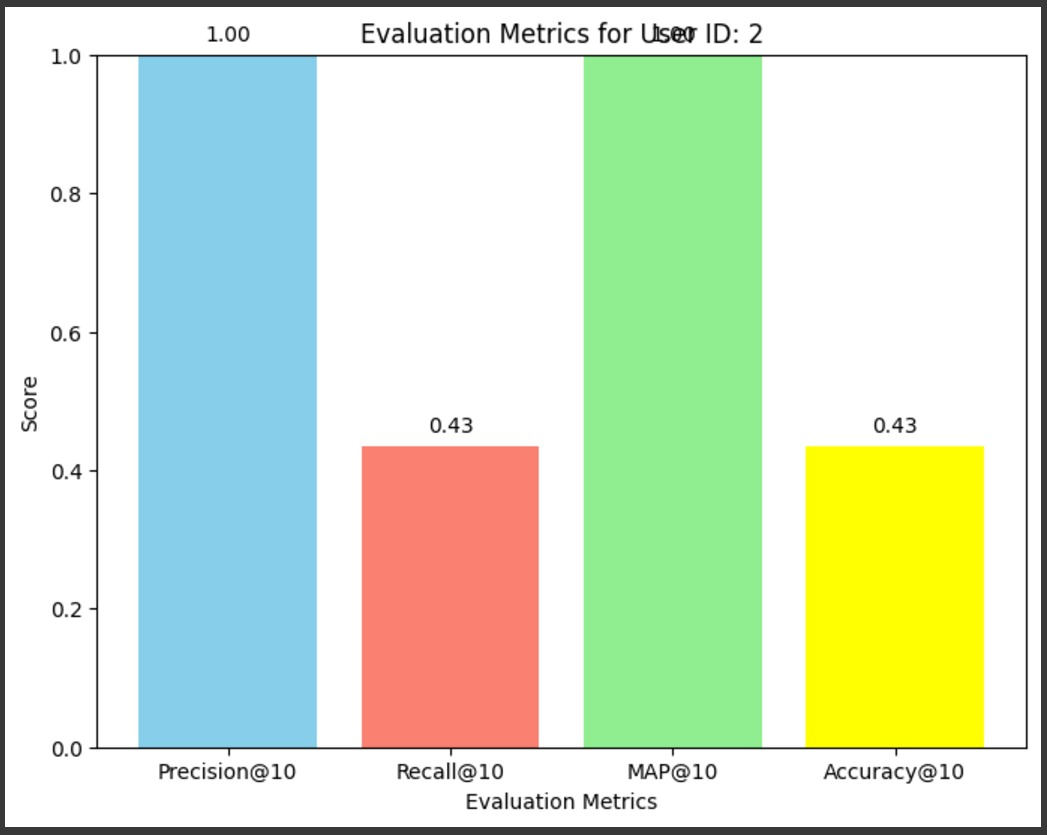
\includegraphics[width=0.6\textwidth]{images/metric1.jpeg}
                \item \textit{Precision@10}: 1.0
                \item \textit{Recall@10}: 0.43
                \item \textit{MAP@10}: 1.0
                \item \textit{Accuracy@10}: 0.43
            \end{itemize}
            \item \textbf{User ID 19}:
            \begin{itemize}
                \item 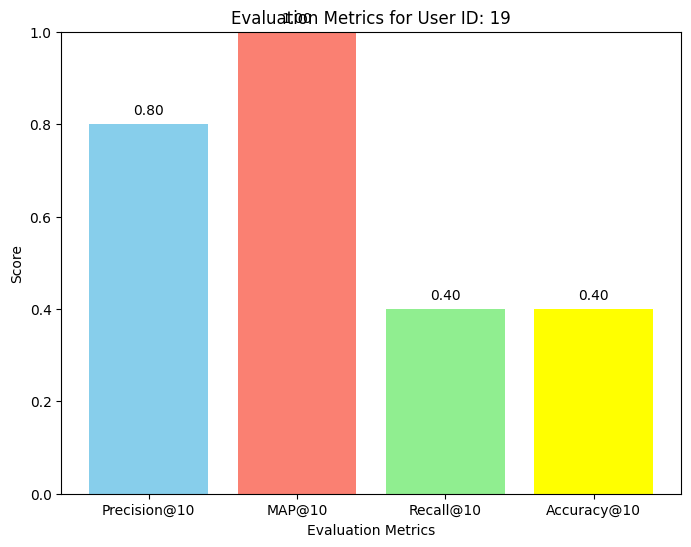
\includegraphics[width=0.6\textwidth]{images/metric2.jpeg}
                \item \textit{Precision@10}: 0.8
                \item \textit{Recall@10}: 1.0
                \item \textit{MAP@10}: 0.4
                \item \textit{Accuracy@10}: 0.4
            \end{itemize}
            \item \textbf{User ID 10}:
            \begin{itemize}
                \item 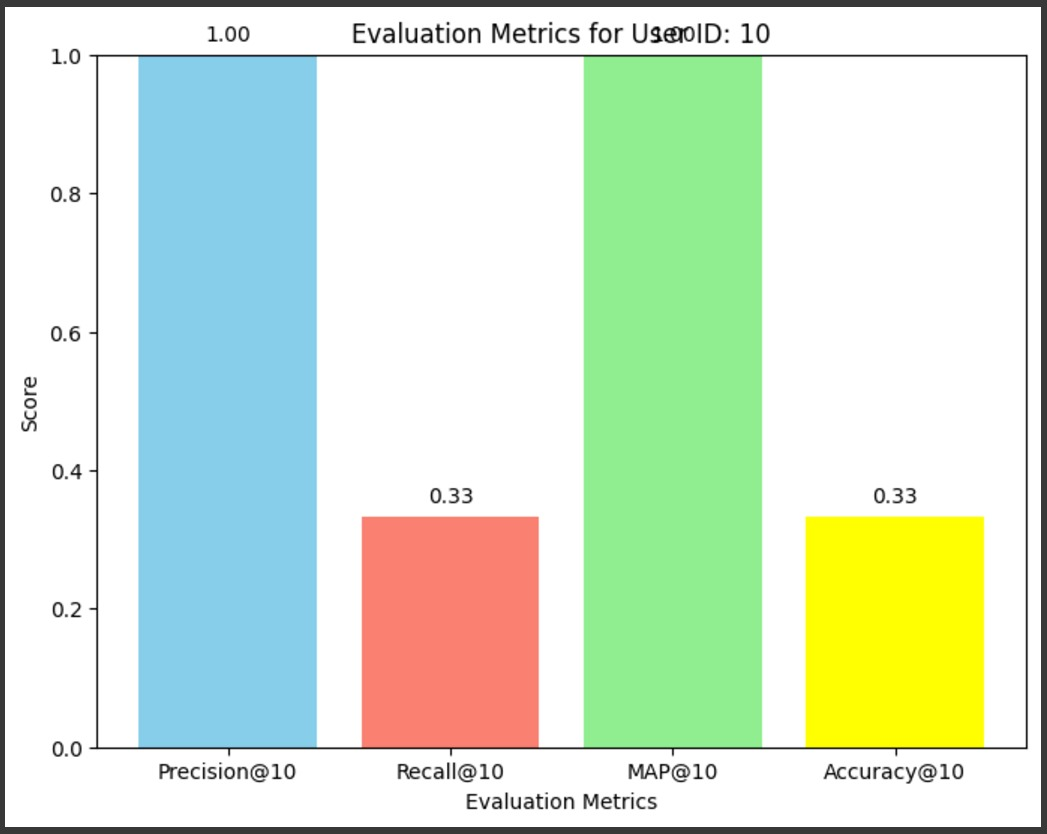
\includegraphics[width=0.6\textwidth]{images/metric3.jpeg}
                \item \textit{Precision@10}: 1.0
                \item \textit{Recall@10}: 0.33
                \item \textit{MAP@10}: 1.0
                \item \textit{Accuracy@10}: 0.33
            \end{itemize}
            \item \textbf{User ID 13}:
            \begin{itemize}
                \item 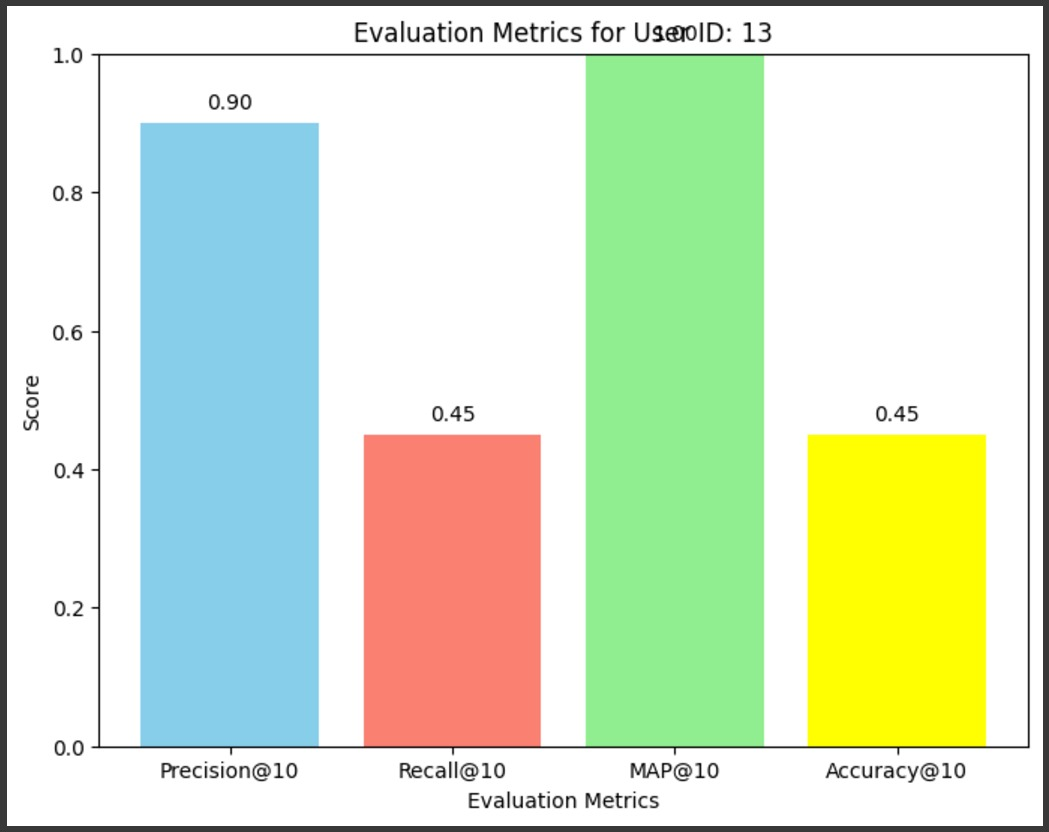
\includegraphics[width=0.6\textwidth]{images/metric4.jpeg}
                \item \textit{Precision@10}: 0.90
                \item \textit{Recall@10}: 0.45
                \item \textit{MAP@10}: 1.0
                \item \textit{Accuracy@10}: 0.45
            \end{itemize}
            \item \textbf{User ID 9}:
            \begin{itemize}
                \item 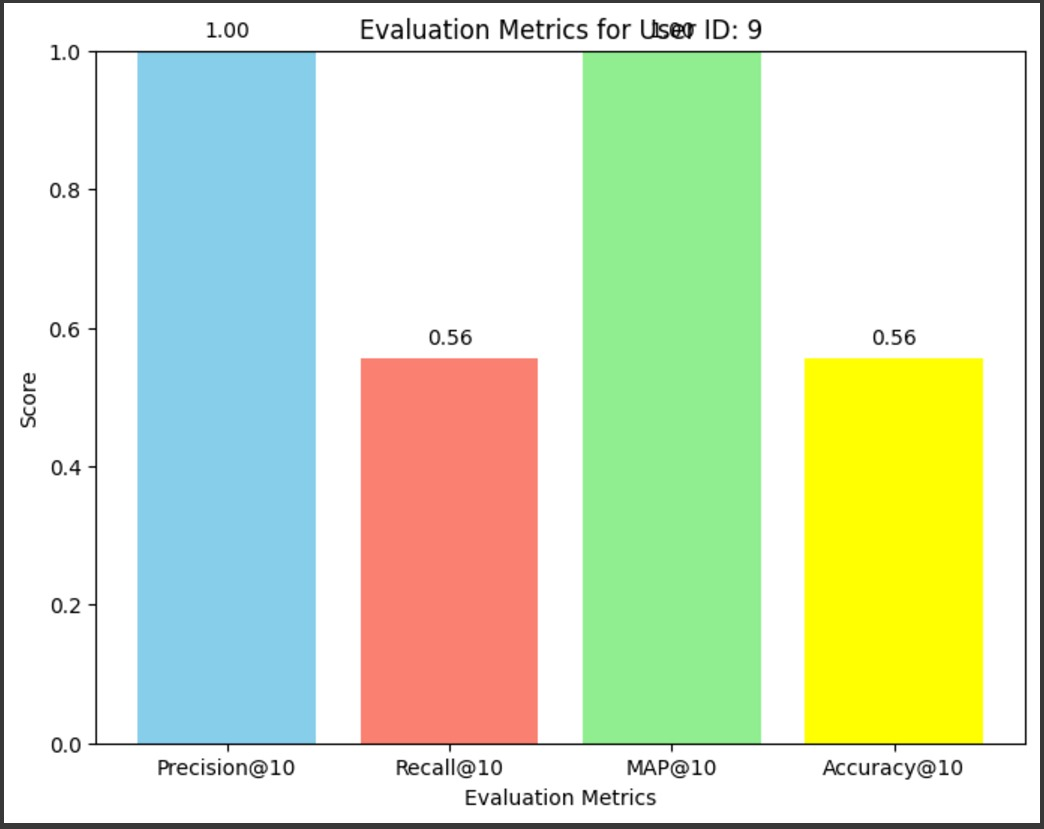
\includegraphics[width=0.6\textwidth]{images/metric5.jpeg}
                \item \textit{Precision@10}: 1.0
                \item \textit{Recall@10}: 0.56
                \item \textit{MAP@10}: 1.0
                \item \textit{Accuracy@10}: 0.56
            \end{itemize}
        \end{itemize}
        
        \item \textit{Simpulan}:
        \begin{itemize}
            \item Setiap modul pengguna menunjukkan variasi dalam metrik evaluasi, yang mencerminkan perbedaan dalam pola interaksi dan preferensi pengguna.
            \item Pengguna dengan riwayat interaksi yang lebih kaya cenderung memiliki nilai precision dan recall yang lebih tinggi, menunjukkan bahwa model dapat memberikan rekomendasi yang lebih akurat.
            \item Variasi dalam MAP dan accuracy menunjukkan bahwa meskipun model memberikan rekomendasi yang relevan, ada ruang untuk peningkatan dalam menangkap semua item relevan.
        \end{itemize}
    \end{itemize}

    \item \textbf{Analisis Kinerja}:
    \begin{itemize}
        \item Model berhasil memberikan rekomendasi yang dipersonalisasi, meningkatkan pengalaman pengguna di platform. Pengguna dengan riwayat interaksi yang lebih banyak mendapatkan rekomendasi yang lebih akurat.
        \item Untuk pengguna baru, model merekomendasikan produk berdasarkan popularitas, memastikan bahwa mereka tetap mendapatkan saran yang relevan meskipun tanpa riwayat interaksi.
    \end{itemize}

% ... existing code ...


\item \textbf{Hasil Tampilan Website}:
\begin{itemize}
    \item \textbf{Antarmuka Pengguna}:
    \begin{itemize}
        \item Antarmuka pengguna dibangun dengan \textit{React.js}, menampilkan produk dan rekomendasi dengan responsif dan interaktif. Pengguna dapat dengan mudah menavigasi dan menemukan produk yang diinginkan.
        \item 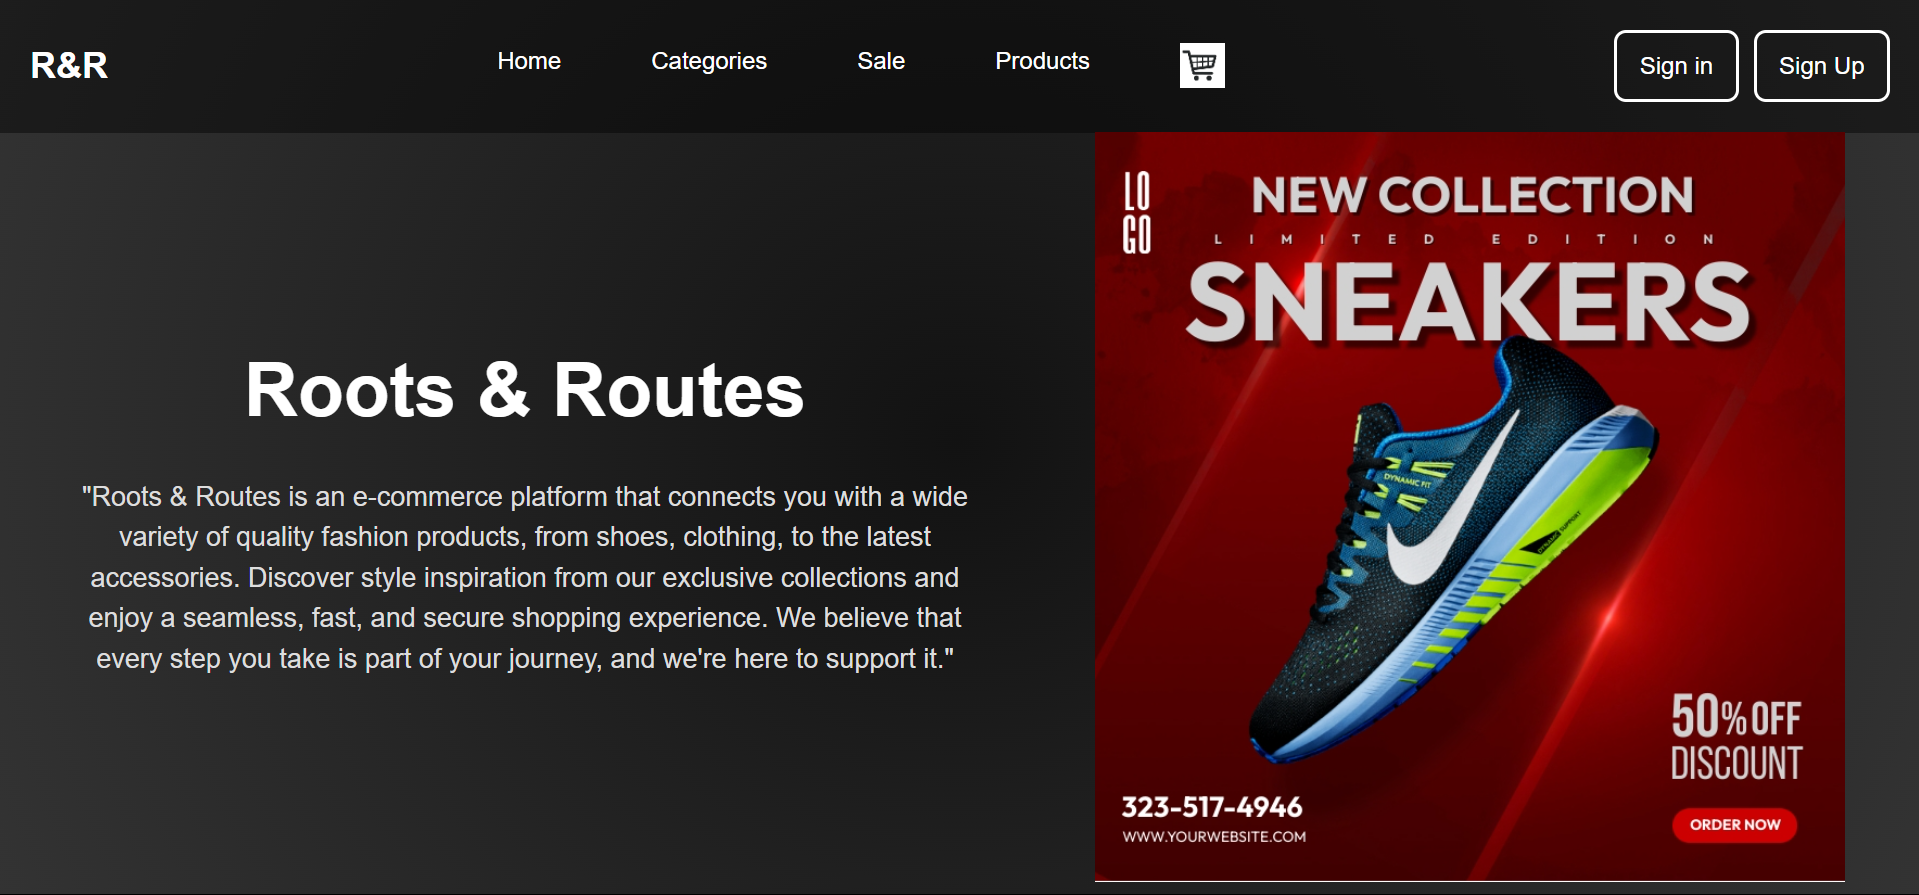
\includegraphics[width=0.45\textwidth]{images/web1.png}
        \caption{Tampilan Halaman Home}
        \item Halaman home menyajikan berbagai kategori produk dan penawaran terbaru, memberikan pengguna akses cepat ke koleksi sepatu yang tersedia.
    \end{itemize}

    \item \textbf{Proses Masuk (Sign In)}:
    \begin{itemize}
        \item 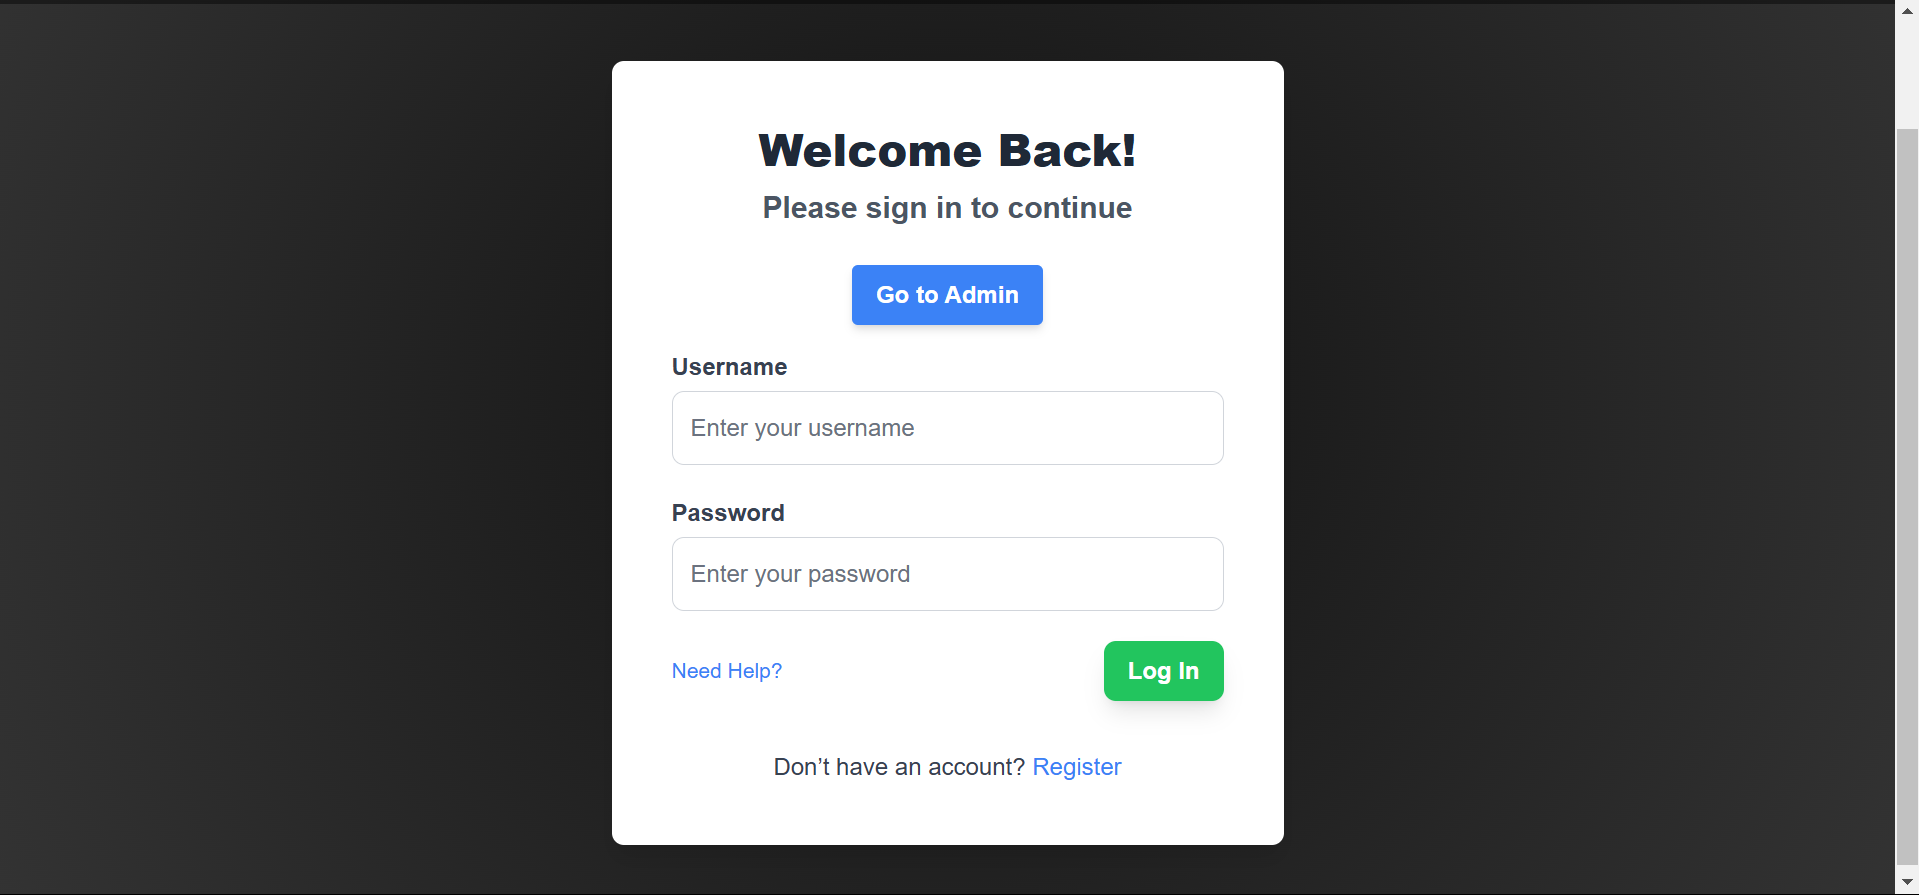
\includegraphics[width=0.45\textwidth]{images/web2.png}
        \caption{Tampilan Halaman Sign In}
        \item Halaman sign in dirancang untuk memudahkan pengguna dalam mengakses akun mereka dengan cepat dan aman, menggunakan form yang sederhana dan intuitif.
    \end{itemize}

    \item \textbf{Daftar Sepatu}:
    \begin{itemize}
        \item 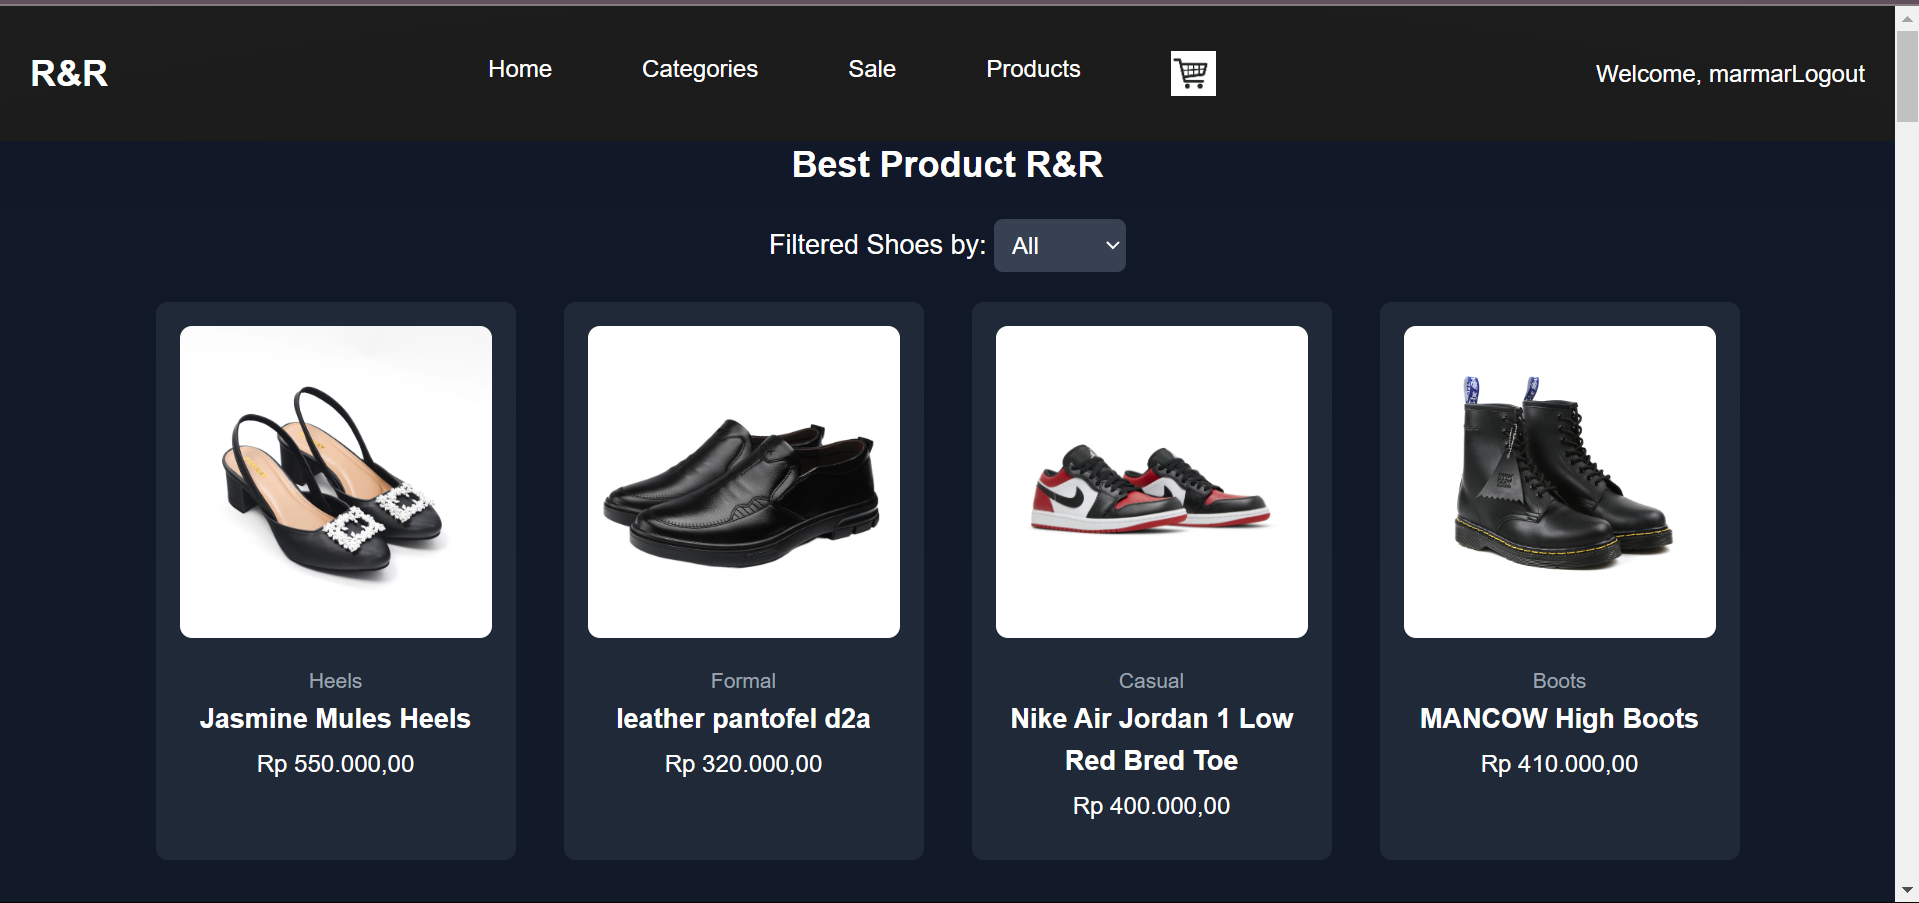
\includegraphics[width=0.45\textwidth]{images/web3.png}
        \caption{Tampilan Daftar Sepatu}
        \item Halaman daftar sepatu menampilkan koleksi sepatu yang tersedia, dilengkapi dengan filter pencarian untuk memudahkan pengguna menemukan sepatu yang diinginkan.
    \end{itemize}

    \item \textbf{Detail Sepatu}:
    \begin{itemize}
        \item 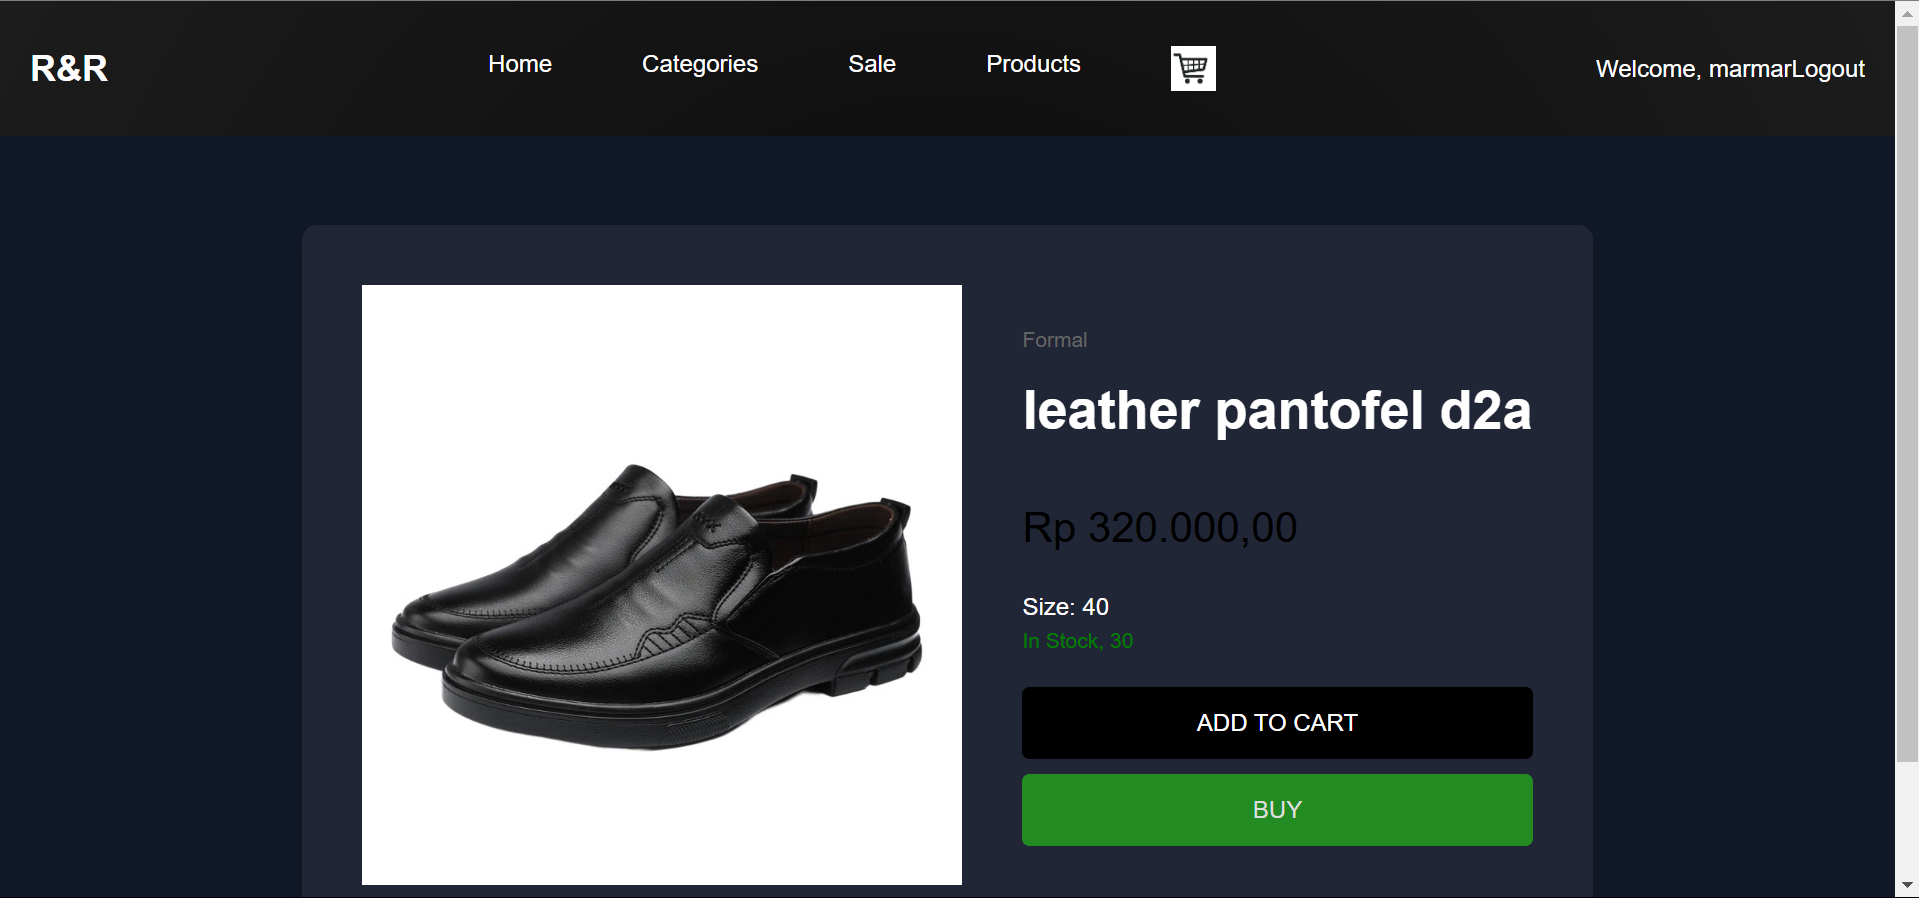
\includegraphics[width=0.45\textwidth]{images/web4.png}
        \caption{Tampilan Detail Sepatu}
        \item Halaman detail sepatu memberikan informasi lengkap tentang produk, termasuk deskripsi, ukuran yang tersedia, dan harga, serta opsi untuk menambahkannya ke keranjang belanja dan opsi beli.
    \end{itemize}

    \item \textbf{Desain UI}:
    \begin{itemize}
        \item Desain UI yang bersih dan intuitif memastikan bahwa pengguna dapat dengan mudah memahami dan menggunakan fitur rekomendasi. Elemen navigasi yang jelas dan tata letak yang terorganisir membantu pengguna dalam menjelajahi produk dan melakukan pembelian.
    \end{itemize}
\end{itemize}

% ... existing code ...



% ... existing code ...

    \item \textbf{Diskusi}:
    \begin{itemize}
        \item \textit{Kekuatan Model}: Model NMF mampu menangkap pola laten dalam data interaksi, memberikan rekomendasi yang relevan dan bervariasi.
        \item \textit{Keterbatasan Model}: Model mungkin kurang efektif untuk pengguna baru dengan sedikit atau tanpa riwayat interaksi. Solusi potensial termasuk menggabungkan data demografis atau menggunakan pendekatan hybrid.
        \item \textit{Peluang Peningkatan}: Mengoptimalkan parameter model dan memperkaya dataset dengan lebih banyak fitur dapat meningkatkan akurasi dan relevansi rekomendasi.
    \end{itemize}
\end{enumerate}

Hasil ini menunjukkan bahwa model rekomendasi yang dikembangkan dapat meningkatkan pengalaman pengguna dan potensi konversi di platform e-commerce, meskipun masih ada ruang untuk perbaikan lebih lanjut.


\subsection{Conclusion}
% Tambahkan konten untuk Conclusion di sini

\section{Appendices (if applicable)}
% Tambahkan konten untuk Appendices di sini

% ... existing code ...

\end{document}